\subsubsection{Spirits}\label{subsubsec:Spirits}
\paragraph{Aufbau}\label{subsubsec:Aufbau_Spirits}\mbox{}\\

Spirits ist eine mobile Cocktailmaschine. Vom Aufbau her hat sie einen Edelstahlkorpus, in welchem die Elektronik, die Pumpen und die Ventile verbaut sind. Um den Korpus herum können die Getränkeflaschen in eine Getränkehalterung hineingestellt werden. Insgesamt haben 8 Flaschen Platz. Diese Kapazität ist jedoch erweiterbar, indem mehrere Maschinen miteinander gekoppelt werden. Ein spezieller Flaschendeckel, durch welchen ein Röhrchen führt, schliesst die Flaschen. Das Röhrchen ist dazu da, die Flüssigkeit aus den Getränkeflaschen zu pumpen. Mit einem Silikonschlauch sind die Röhrchen mit dem Korpus verbunden. Auf der Frontseite ist ein Touch-Display verbaut, über welchem sich eine Abstellmöglichkeit für ein Glas befindet. Darüber befindet sich der Flüssigkeitsauslass. Auf der Rückseite befinden sich diverse Anschlüsse wie 2x USB, 1x Ethernet, 2x Chinch R+L, 1x Artnet\footnote{Artnet=Kommunikationsprotokoll für intelligente Scheinwerfer, Moving Heads und Effektgeräte (Remote Device Management)} und die Stromversorgung. \cite{koths_spirits_nodate}

\paragraph{Bedienung}\label{subsubsec:Bedienung_Spirits}\mbox{}\\

Die Bedienung kann neben dem Display auch über ein Smartphone, ein Tablett oder einen PC geschehen. Kommuniziert wird dabei über das eigene WLAN-Netz der Spirits-Cocktailmaschine, welche somit als Accesspoint dient. Sobald die Bestellung eingegangen ist, reicht es ein mit Eis gefülltes Glas unter den Flüssigkeitsauslass zu stellen und das Getränk zur Zubereitung freizugeben.\cite{koths_spirits_nodate}

\newpage


\paragraph{Technische Daten}\label{subsubsec:Technische_Daten_Spirits}\mbox{}\\

\begin{tabular}{@{}llp{0.6\textwidth}}
    Zeit für einen Cocktail: & : & Aufgrund paralleler Getränkeförderung braucht der Spirits nur ca. 20s, um 3dl eines Cocktails zu erstellen. \cite{koths_spirits_nodate}\\
    \hline
    Anzahl verschiedene Cocktails: & : & Abhängig von den Mischgetränken und benötigten Zutaten. Sind mehrere Cocktails erwünscht, können im Betrieb die Zutaten getauscht werden oder mehrere Spirits miteinander verknüpft werden. \cite{koths_spirits_nodate}\\ 
    \hline
    Stromversorgung: & : & In Spirits ist ein Akku verbaut, so dass die Maschine auch ohne Steckdose verwendet kann. Zum Aufladen des Akkus und für den Dauerbetrieb benötigt sie jedoch eine Steckdose. \cite{koths_spirits_nodate}\\
\end{tabular}

\paragraph{Reinigung}\label{subsubsec:Reinigung_Spirits}\mbox{}\\

Zur Reinigung können alle Schläuche in ein mit heissem Wasser gefüllten Gefäss hineingelegt werden. Weiter muss ein leeres Gefäss unter den Flüssigkeitsauslass gestellt werden. Über die App kann nun das Reinigungsprogramm aufgerufen werden. Nun befördern die Pumpen das heisse Wasser durch die Schläuche und reinigen alles. Nach dem Vorgang die Schläuche aus dem Wasser nehmen und nochmals laufen lassen, damit die Pumpen das restliche Wasser aus den Schläuchen Pumpen.
Bevor die Reinigung jedoch gestartet wird, kann die noch in den Schläuchen befindende Flüssigkeit in die Behälter zurück gepumpt werden.\cite{koths_spirits_nodate}

\paragraph{Sonstiges}\label{subsubsec:Sonstiges_Spirits}\mbox{}\\

Spirits kann sogar Musik abspielen. Es ist möglich, eigene Playlists zu erstellen und zu beeinflussen. Die Musik kann auf USB-Sticks, auf externen Festplatten oder auf dem internen Speicher abgelegt und aufgerufen werden. Mittels Voting können die Anwesenden den Musikverlauf steuern. Auch Lichteffekte sind mit Spirits möglich. So können DMX\footnote{DMX=Digitales MultipleX}-Geräte über das Artnet-Protokoll gesteuert werden. Diverse Lichtprogramme sind schon hinterlegt. Weitere Lichtszenen können angelegt und gespeichert werden. Von Spirits gibt es drei verschiedene Ausgaben, welche sich jedoch rein darin unterscheiden, dass sie unterschiedliche Getränkehalterungen haben.\cite{koths_spirits_nodate}

\begin{figure}[h]
	\centering
	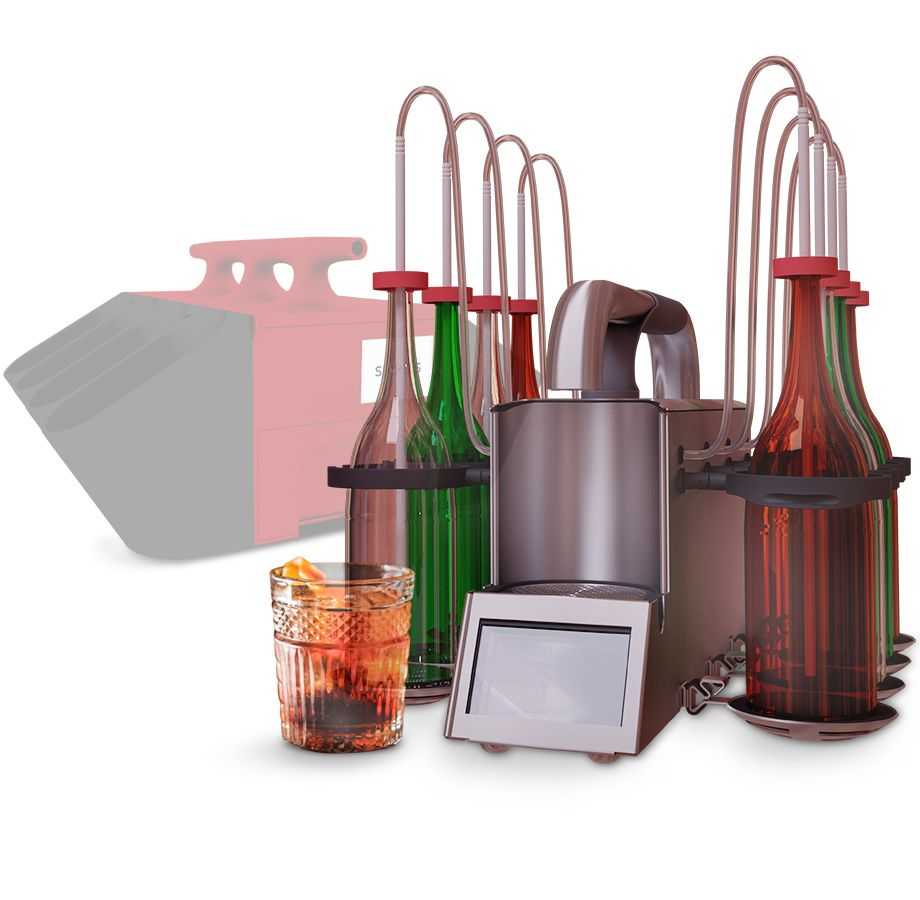
\includegraphics[width=0.35\textwidth]{graphics/Spirits.JPG}
	\caption{Spirits-Cocktailmaschine \cite{koths_spirits_nodate}}
	\label{fig:Spirits_Cocktailmaschine}
\end{figure}